\documentclass{ecai2014}

% Parts of the style depend on whether a PDF or a DVI output is created.
\usepackage{ifpdf}

\usepackage{algorithms}
\usepackage{amsfonts}
\usepackage{amsmath}
\usepackage[english]{babel}
\usepackage{graphicx} % Also in ECAI 2014 example document.
\ifpdf
  % Declare the supported file extensions.
  \DeclareGraphicsExtensions{.jpg,.pdf,.png}
\fi
\usepackage{latexsym} % Also in ECAI 2014 example document.
\usepackage{times} % Also in ECAI 2014 example document.
\usepackage{url}
\usepackage{verbatim}

\newcommand{\tn}{\textnormal}
\newcommand{\ts}{\textsf}
\newcommand{\B}{{\mathbb B}}
\newcommand{\X}{{\mathcal X}}
\newcommand{\Y}{{\mathcal Y}}
\newcommand{\U}{{\mathcal U}}
\newcommand{\M}{{\mathcal M}}
\renewcommand{\B}{{\mathcal B}}
\renewcommand{\L}{{\mathcal L}}
\newcommand{\T}{{\mathcal T}}
\newcommand{\D}{{\mathcal D}}
\renewcommand{\P}{{\mathcal P}}
\newcommand{\I}{{\mathcal I}}
\newcommand{\half}{\tfrac{1}{2}}
\newcommand{\ind}{\mathop{\mathbf{1}}}
\newcommand{\class}{\tn{class}}
\newcommand{\first}{\tn{first}}
\newcommand{\refs}{\tn{refs}}
\newcommand{\splt}{\tn{split}}
\newcommand{\find}{\tn{find}}
\newcommand{\tuple}[1]{{\left\langle{#1}\right\rangle}}
\newcommand{\concat}{\oplus}

\newcommand{\triple}[3]{\langle#1,#2,#3\rangle}
\newcommand{\pair}[2]{\langle#1,#2\rangle}

% Theorem styles.
\newtheorem{assumption}{Assumption}
\newtheorem{axiom}{Axiom}
\newtheorem{convention}{Convention}
\newtheorem{example}{Example}
\newtheorem{definition}{Definition}
\newtheorem{lemma}{Lemma}
\newtheorem{principle}{Principle}
\newtheorem{proposition}{Proposition}
\newtheorem{specification}{Specification}
\newtheorem{statement}{Statement}
%\newtheorem{theorem}{Theorem}

\newcommand{\Parameters}{\textbf{additional parameters} }

\newcommand{\Psm}[1]{\tn{P}_{\tn{sm}(#1)}}
\newcommand{\Pkt}[1]{\tn{P}_{\tn{kt}(#1)}}
\renewcommand{\Pr}{\tn{P}_\tn{r}}

\smallalgo

\begin{document}

\title{
  Schema-based Partitioning of Resources\\
  using MDL Model Selection
}

\author{Steven de Rooij \and Wouter Beek \and Stefan Schlobach\footnote{
  VU University Amsterdam}}

\maketitle

\begin{abstract}
Clustering resources into different kinds can be useful
 for various purposes, e.g. browsing based on categories,
 providing automatic suggestions for ontology design.
Existing approaches towards partitioning a set of resources
 have shortcomings.
They either identify too few partition members
 given the data at hand,
 or they identify too many partition members
 than can be substantiated by the data. 
We define a generalization of these existing approaches
 and show that a more granular partition can be found
 that is still validated by the data, i.e. that do not overfit.
\end{abstract}

\section{Introduction}
\label{sec:intro}
\label{sec:relwork}

Clustering resources into different kinds can be useful
 for various purposes, e.g. browsing based on categories,
 providing automatic suggestions for ontology design.

We argue that RDF data deals with resources of different ``kinds'':
 two resources of the same kind will have similar relations
 to other resources.
We exploit this to partition the data into ``kinds'' automatically.

There are various ways to partition a set of resources into kinds.
The most straightforward approach is to use an explicit vocabulary
 in order to indicate
   that resources are members of the same set (extensional definition)
 or
   that resources are instance of the same class (intensional definition).
The vocabulary of RDF(S) \cite{BrickleyGuha2014} uses
 the intensional definition,
 denoted by the \texttt{rdf:type} property term.

In addition to used the explicit schema information,
 various methods have been explored that
 extract implicit schema information.
In \cite{NeumannMoerkotte2011},
 kinds of resources are identified
 by their \emph{characteristic set},
 which is the set properties that are asserted of a resource.

A comparison of the type-based and the property-based
 identification of resource kinds was performed by \cite{GottronKSS13},
 who showed that there is considerable mutual information between
 these two approaches.

A third approach is to use the object terms in addition to the predicate terms
 in order to characterize a resource.
In \cite{buikstra2011ranking}, the similarity between two resources
 is measured by the number of predicate-object pairs they have in common.

As we will argue in Section \ref{sec:fingerprints},
 the existing approaches towards partitioning a set of resources
 have shortcomings: they either identify too few partition members
 given the data at hand, or they identify too many partition members
 than can be substantiated by the data. 

In Section \ref{sec:approach} we give a generalization of
 these existing approaches and show that for arbitrary datasets
 more granular partitions can be found that are still validated
 by the data, i.e. that do not overfit.
Section \ref{sec:implementation} gives some implementation details,
 and Section \ref{sec:evaluation} shows the evaluation results we
 obtained by executing our implementation on existing datasets.
Section \ref{sec:conclusion} concludes.


%\section{Related work}
\label{sec:related_work}

Existing research suggests six different solutions for
  the problem of identity on the SW.

\textbf{[1] Introduce weaker versions of {\small \texttt{owl:sameAs}}}
  \cite{HalpinHayes2010,MccuskerMcguinness2010}.
Candidates for replacement are
  the SKOS concepts
  {\small \texttt{skos:related}} and {\small \texttt{skos:exactMatch}}
  \cite{MilesBechhofer2009}.
The former is not transitive,
  thereby limiting the possibilities for reasoning.
The latter is transitive,
  but can only be used in certain contexts.
It is not defined in what contexts it can be used
  \cite{MilesBechhofer2009}.\footnote{
    For instance, the property {\small \texttt{skos:exactMatch}}
    ``is used to link two concepts, indicating a high degree of confidence
    that the concepts can be used interchangeably across a wide range of
    information retrieval applications.''
  }
\begin{comment}
% SIMILARITY
The problem with using weaker notions such as relatedness,
  is that everything is related to everything in \emph{some} way.}
% Shall we discuss similarity here as well?
% Does similarity differ from relatedness?
\end{comment}

\textbf{[2] Restrict the applicability of identity relations}
  to specific contexts.
In terms of Semantic Web technology, identities are expected to hold
  within a named graph or within a namespace,
  but not necessarily outside of it \cite{HalpinHayes2010}.
\cite{Melo2013} has successfully used the Unique Names Assumption
  within namespaces in order to identify many (arguably) spurious
  identity statements.

\textbf{[3] Introduce additional vocabulary} that does not weaken but extends
  the existing identity relation.
\cite{HalpinHayes2010} mention an explicit distinction that could be made
  between mentioning a term and using a term,
  thereby distinguishing an object and a Web document describing that object.
Other possible extensions of {\small \texttt{owl:sameAs}} might take
  the Fuzzyness and/or uncertainty of identity statements into account.

\textbf{[4] Use domain-specific identity relations}
  \cite{MccuskerMcguinness2010}.
For instance
    ``$x$ and $y$ have the same medical use''
  replaces
    identity in the domain of medicine,
and
    ``$x$ and $y$ are the same molecule''
  replaces
    identity in the domain of chemistry.
The downside to this solution is that domain-specific links are
  only locally valid, thereby limiting knowledge reuse.

\textbf{[5] Change the modeling practice}, possibly in a (semi-)automated way
  by adapting visualization and modeling toolkits to produce notifications
  upon reading SW data, or by posing additional restrictions on the creation
  and alteration of data. For example, adding an RDF link could require
  reciprocal confirmation from the maintainers of the respective datasets.
  \cite{HalpinHayes2010,DingShinavierFininMcguinness2010}
The problem with introducing checks on editing operations,
  is that it violates one of the fundamental underpinnings of the SW;
  namely that on the Web of Data anybody is allowed to say
  anything about anything \cite{AntoniouGrothHarmelenHoekstra2012}.

\textbf{[6] Extract network properties of {\small \texttt{owl:sameAs}}
  datasets} \cite{DingShinavierShangguanMcguinness2010}.
Although this work shows that network analysis can provide insights
  into the ways in which identity is used in the SW,
  these endeavors have not yet been related to the semantics of the
  identity relation.
We believe that utilizing network theoretic aspects in order to
  determine the meaning of identity statements
  would be interesting future research.

What the existing approaches have in common is
  that quite some work has to be done
  (adapting or creating standards, instructing modelers, converting existing
  datasets) in order to resolve only some of the problems of identity.
Our approach provides a way of dealing with the heterogeneous real-world
  usage of identity in the SW that is fully automated and requires
  no changes to standards, modeling practices, or existing datasets.


\section{Fingerprints for identifying kinds}
\label{sec:fingerprints}

The ``kind'' of a resource is identified by a fingerprinting technique.
We first define the existing fingerprint techniques
 (see Section \ref{sec:relwork})
 in a uniform way, and then define our own technique,
 which is a generalization of the existing methods.

We use $G$ to denote a graph, i.e. an arbitrary set of triples
The set of subject, predicate, and object terms that occur in $G$
 are denoted by $S_G$, $P_G$, and $O_G$ respectively.
A fingerprint is then a function $f : S_G \rightarrow \mathcal{P}(O_G)$
 such that the equivalence relation characterized by $f$
 (equation \ref{def:eq}) induces a partition on $O_G$
 that distinguishes between different kinds of resources.

\begin{definition}
  \label{def:eq}
  For an arbitrary fingerprint function $f$,
   the partition induced by $f$ is $\{ [s]_{\approx} \mid s \in S_G \}$,
   where $\approx \,\, = \{ \langle s, s' \rangle \in S_G^2 \mid f(s) = f(s') \}$.
\end{definition}

We identify subsets of RDF terms based on
  their positional occurrence in triples in $G$:
  $S_G$, $P_G$, and $O_G$ denote the subject, predicate and object terms
  in $G$ respectively.

The interpretation $I$ maps RDF terms onto resources,
  and triples onto truth values.
The extension function $Ext$ maps resources onto pairs of resources.
$I(\triple{s}{p}{o})$ is true iff
  $\pair{I(s)}{I(o)} \in Ext(I(p))$ \cite{Hayes2014}.

The first candidate for the fingerprint (called $f_1$)
 identifies kinds in terms of the set of classes
 of which a given resource is an instance (definition \ref{def:class}).
The usefulness of this method depends on
 the availability of explicit `instance-of' predications in the data.

\begin{definition}[Approach using classes]
  \label{def:class}
  $f_1(s) = \\
  \{ c \mid I(s) \in Ext(I(c)) \}$
\end{definition}

The second approach for the fingerprint (called $f_2$)
 identifies kinds in terms of the set of shared predicates
 (definition \ref{def:predicate}).
This approach has drawbacks in those cases in which the property occurs
 for resources of different kinds.
An example is 

\begin{definition}[Approach using predicate terms]
  \label{def:predicate}
  $f_2(s) = \\
  \{ p \mid \exists o: \langle I(s), I(o) \rangle \in Ext(I(p)) \}$
\end{definition}

The drawback of this method is that it cannot distinguish between
 different kinds that have the same properties,
 i.e. it missed out on a potentially relevant granularity level:
 the object terms that occur in the predicate extension.
For instance, in a dataset that consists of personal profiles,
 most resources may be the property ``gender'' defined,
 but the distinction between the kinds male and female persons
 can only be made when the object terms ``male'' and ``female''
 are known as well.

The third candidate for the fingerprint (called $f_3$)
 identifies kinds in terms of the set of shared predicate-object pairs
 (definition \ref{def:po_pairs}).

\begin{definition}[Approach using predicate-object pairs]
  \label{def:po_pairs}
  \[
    f_3(s)
  =
    \{
      \langle p, o \rangle \in P_G \times O_G
    \mid
      \langle I(s), I(O) \rangle \in I(p)
    \}
  \]
\end{definition}

Including the object terms in the fingerprint solves the granularity problem:
 now
  resources with male gender
 can be distinguished from
  resources with the female gender.
But by including every object in the fingerprint,
 the granularity level may be too fine-grained,
 inviting over-fitting.
In these cases the object terms are too specific to give
 useful information about the kind of its related subject term.
%For example, if another predicate in the database of personal profiles
% is \texttt{foaf:family\_name},
% then each resource has a different type as identified by $\psi$.
For example, in a dataset describing a social network
 there will be many people who are intuitively of the same kind
 (people living in the UK, people who went to the same high school),
 even though they may not share any friends.

We conclude that it is sometimes useful to include the object term
 in the fingerprint, but this is not always so.
In the next section we introduce an approach that allows us
 to automatically determine when an object is useful to be included
 in the fingerprint and when it is no longer useful to do so,
 i.e. when overfitting occurs.


\section{Approach}
\label{sec:approach}

In contrast to the explicit schema information that should be present
in an RDF data set in the form of \texttt{rdf:type} specifications, in
this section we will use the structural properties of the graph to
extract implicit schema information.
structural properties of the graph can be used

In the previous section we saw that both excluding and including object terms
 in the partitioning of resources has negative effects on some data.
In this section we seek the best of both worlds
 and generalize these approaches using a partition $\M$ of resources.

Let $\tn{class}(t) = C$ iff $t \in C$ and $C \in \M$,
 thus the class of a term is its partition cell.
We now define the generic fingerprint (called $f_\M$) of a subject term $s$
 in Definition \ref{def:fingerprint}.

\begin{definition}[Fingerprint]
  \label{def:fingerprint}
  $
    f_\M(s)
  := \\
    \{
      \tuple{p,C} \in P_G \times \mathcal{P}(O_G)
    \mid
      \pair{I(s)}{I(o)} \in Ext(I(p)) \, \wedge \, o \in C \\
      \wedge \, C \in \M
    \}
  $
\end{definition}

The fingerprints $f_2$ and $f_3$ in Section \ref{sec:fingerprints}
 are instantiations of the generic fingerprint $f_\M$.
They correspond to, respectively,
  a partition $\M$ that contains a single set of all terms,
 and
  a partition $\M$ that contains all terms as singleton sets.

The advantage of generalizing these methods using $f_m$ is that
 a well chosen $\M$ can interpolate between these two existing approaches,
 and retain all relevant information about the term while discarding
 irrelevant details.
Our method of selecting a suitable partition is
 described in Section~\ref{sec:mdl} below.

\subsection{MDL Model Selection}
\label{sec:mdl}

A well motivated approach to model selection is based on
 the Minimum Description Length (MDL) principle
 \cite{Rissanen78,Rissanen84,grunwald2007}.
MDL can be interpreted as a formalization of Occam's Razor,
 which states that a more simple hypothesis,
 or model, should be preferred over a more complicated explanation of
 the same data.
In MDL, the words ``simple'' and ``complicated'' are
 made precise by using codes.
Given a space $\M$ of models, and data $D\in\D$,
 we have to specify:

\begin{itemize}
\item A code $C:\M\to\{0,1\}^*$ to encode the model
\item For each model $M\in\M$, a code $C_M:\D\to\{0,1\}^*$ to encode
  the data, making use of the model.
\end{itemize}

The second code uses the model in order to achieve an efficient encoding.
The best model is then the one that minimizes the overall code-length
 (equation \ref{eq:mdl}).

\begin{equation}
  \label{eq:mdl}
  M_\tn{mdl}:=\arg\min_{M\in\M}|C(M)| + |C_M(D)|.
\end{equation}

By balancing these two contributions
 (the coder and the data encoded using that codes)
 to the code length,
 MDL avoids very simple models that provide poor fit to the data
 (as these would have a long $C_M(D)$),
 and it also avoids overfitting,
 as overly complex models have a long $C(M)$.
Also note that the model selection procedure only relies on
 the code \emph{lengths}, so it suffices to define code length functions
 without worrying about the actual code words.
In the following we will write $L(x)$ as a shorthand for $|C(x)|$.

MDL model selection is very closely related to Bayes factors model selection,
 where the prior distribution on models replaces $C(M)$
and the likelihood function replaces $C_M(D)$;
readers more familiar with Bayesian methodology may wish to
 mentally make these substitutions and reading
 ``negative loglikelihood'' wherever we write ``code length''.

In our application,
 the model $\M$ is the partition that determines the fingerprints.
The construction of the code is outlined in the next section.




\section{Implementation}
\label{sec:implementation}

Using our operationalization of the five star model of data sharing
 in section \ref{sec:operationalization} we created
 a web observatory for linked open data,
 called \obs.\footnote{Code and results available at
   \url{https://github.com/wouterbeek/LODObs}}

\obs uses an automated script in order to look for
 data on the Web.
The script must be given a set of locations where Web data
 is likely to be found.
For this we use CKAN API.\footnote{\url{http://docs.ckan.org}}
CKAN is an open-source data portal platform
 that allows datasets that are published on the Web to be catalogued.
There are various catalogues available,
 including the governmental initiatives towards data sharing
 of the UK and the USA.

\obs gives a tabular overview of the results of
 processing the various resources, see Figure \ref{fig:lod_observer}.
\obs provides more detailed information than we are able to give
 in our results section (i.e. section \ref{sec:results});
 e.g. it shows the specific error messages encountered
 and the syntax error that occur while reading a serialization format.

\begin{figure*}[th!]
  \label{fig:lod_observer}
  \centering
  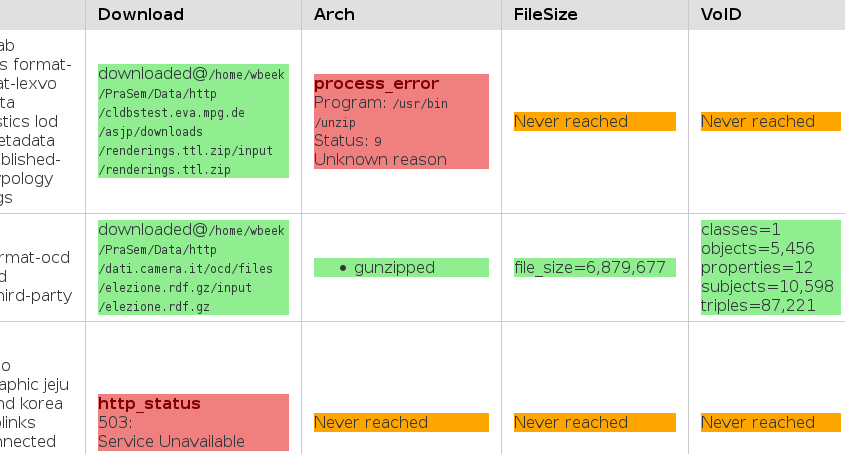
\includegraphics[width=0.85\textwidth]{./img/table}
  \caption{
    A part of the table that is generated by \obs.
    Each row in the table displays the results of retrieving a single
     resource from Datahub.
    Each column in the table corresponds to a specific action
     that is performed for a specific resource.
    The picture shows the results of executing the following four actions
     for three resources:
     (1) downloading the resource,
     (2) unarchiving it,
     (3) determining the file size, and
     (4) counting some basic VoID statistics \cite{Void2011}.
  }
\end{figure*}

\subsubsection*{Locating resources}

CKAN uses URLs as universal locators for resources.
URLs are URIs that identify a resource via a representation of
 its primary access mechanism or scheme (e.g. HTTP)
 and its network location (e.g. \texttt{www.datahub.io})
 that can be accessed using standardized operations
 defined for that scheme. \cite{Rfc3305}

The datasets that are catalogued by CKAN provide
 a starting point for an automated agent to search for data on the Web,
 since all data registrations can be queried using an API.
Since datasets have to be explicitly registered at a CKAN catalogue,
 this ensures that they are purposefully published
 as machine-processable data,
 thereby following our definition of a `resource'
 (see section \ref{sec:operationalization})
Each CKAN resource has a URL property field,
 which allows an automated agent to find a URL string for each resource.

\subsubsection*{Connecting to disseminating host}

When using the URL string to locate a resource we find that
 not all URL strings parse according to the grammar
 in the URL specification \cite{Rfc3986},
 and some URLs that are grammatically correct contain a scheme
 that is not registered with
 the Internet Assigned Numbers Authority
 (IANA).\footnote{\url{http://www.iana.org/assignments/uri-schemes/uri-schemes.xhtml}}
%\footnote{
%  The number of resources for which the URL string parses correctly
%  can be increased by trimming leading and trailing whitespace (US-ASCII 32)
%  and by prepending the string with a commonly occurring scheme descriptor
%  (e.g., \texttt{http://}) in case the grammar cannot detect a scheme.
%}

Culprits:
\begin{itemize}[noitemsep,nolistsep]
  \item The URL string does not parse according to the RFC grammar.
  \item The parsed URL string does not contain an IANA-registered scheme.
\end{itemize}

For URLs that are grammatically correct an automated agent is able to
 verify whether there exists a host authority at the location
 denoted by the URL.
As with the Web of Documents, this is not always the case,
 resulting in a ``host not found exception''.
Once a host authority is found, it has to accept a connection
 with the automated agent.
Only when a connection is established can the agent send its request
 to the authority.
The agent and authority both have to maintain the connection
 for the duration of the subsequent request/response-interaction.

Culprits:
\begin{itemize}[noitemsep,nolistsep]
\item The host that is denoted by the URL's authority string cannot be found.
\item The connection was refused by the host.
\item The connection was neither refused nor accepted by the host.
\item The connection was established, but was broken off
      during subsequent communication.
\item The host was redirecting the connecting agent indefinitely.
\end{itemize}

\subsubsection*{Retrieving resource from host}

Once a reliable connection between agent and host is established
 for the duration of a communicative interaction,
 the agent is able to send a request in one of
 the standardized Internet communication protocols.
Specifically, \obs supports communications via FTP and HTTP(S).

Various things can go wrong in both formulating the request and
 in replying to it.
This results in various status codes that denote different problems
 that cause the communication to be ineffective.

\subsubsection*{Open license}

Many CKAN registered resources have a license property.
The licenses are similar to those defined by the Open Data Commons,
 but some mismatches occur.
In the Datahub CKAN repository, 33 licenses are used,
 18 of which are underdefined (i.e., with no semantic description),
 impacting 5\% of the resources.
We have added manual mappings from the CKAN licenses onto
 the repository of Open Data Commons license descriptions.
%This results in added descriptions for 14 underdefined licenses,
% additional properties for 4 licenses that were already partially defined,
% and leaves only 2 underdefined licenses that have been equated to
% `license' \texttt{ckan:None} using \texttt{owl:sameAs} statements.

Culprits:
\begin{itemize}[noitemsep,nolistsep]
\item Has no license string.
\item Has a license string that cannot be mapped to
       a license that occurs in
       the Open Data Commons license description set.
\item Has a recognized license that is not open.
\end{itemize}

\subsubsection*{Structured \& non-propetary}
\label{sec:implementation_mime}

In order to implement the structuredness requirement,
 we have manually classified the MIME types that occur in the CKAN catalogue
 into `structured' and `unstructured' ones.
This goes against our interpretation of structuredness as
 a gradient property, but the partial order constituted by the relation
 ``supports at least the same set of relational operators''
 cannot be easily established in an automated way,
 as this would require a model of query operators
 and a description of MIME types in terms of the operators that are
 supported by those content types.

We list the 4 ways in which we can check for a resource's content type
 in CKAN, annotated with the number of resources for which
 this type can be retrieved:
\begin{itemize}[noitemsep,nolistsep]
  \item The value of the CKAN \texttt{mimetype} property.
        Present for 6,332 resources (45\%).
  \item The value of the CKAN \texttt{format} property
        Present for 10,226 resources (73\%).
  \item The MIME type in the HTTP \texttt{Content-Type} response header
         (not present in CKAN).
  \item The extension of the resource file.
\end{itemize}

We are specifically interested in linked data,
 but not all linked data serialization formats have a MIME type
 that is registered by IANA.
Moreover, some of the registered linked data content types are deprecated.
We take both deprecated and current MIME types into account,
 and officially registered ones as well as ones that are
 de facto being used to denoted linked data.
Not all MIME types that occur in CKAN repositories are valid,
 some of them seem to be typos/variants of existing MIME types
 for which we have added mappings manually.

The values of the CKAN \texttt{format} property are not standardized
 and are also manually mapped onto IANA-registered and de facto used
 MIME types.
Some of the format values seem to be typographic variants
 of each other (impacting 96 resources).
For some format values no mapping to an existing MIME type
 could be found (impacting 52 resources).

%The MIME type that occurs in the \texttt{Content-Type} response header
% is not always the same as the MIME type denoted by either the
% \texttt{format} or the \texttt{mimetype} property.
%Sometimes this is more generic or a more specific than
% the CKAN-registered value (XX\%),
% but sometimes it is another value altogether.

File extensions were not mapped to content type,
 because of the absence of a straightforward mapping.
We do not believe file extensions are a reliable indicator
 of a resource's format.

A special case occurs for resources that are compressed
 in some archive format.
For these neither MIME type, format, nor Content-Type header
 are indicative of the uncompressed content,
 so for these we have to rely on the file extension.

When none of the above enumerated methods works,
 we can try to parse a file's first few lines.
This is generally quite difficult because of the large number
 of different formats, encoding types, and syntactic error that may occur.
In the general case we are only able to make a best guess at
 a resource's format.

Culprits:
\begin{itemize}[noitemsep,nolistsep]
  \item The resource's type is not set.
  \item The resource's type is set, but it does not map to a MIME type
         that is registered by IANA and it is not one of the MIME types
         in the list of de facto used identifiers of LOD content.
  \item The resource's type can be mapped to an IANA-registered type
         or a de facto LOD type, but it does not denote structured data.
  \item The resource's type can be mapped to an IANA-registered type
         or a de facto LOD type, but it denotes a proprietary format.
\end{itemize}

\subsubsection*{Syntactic correctness: readable triples}

We use SWI-Prolog's Semweb library \cite{wielemaker2003}
 for loading the resources into a triple store.

The number of triples that can be loaded is often inconsistent with
 the value of the CKAN \texttt{size} property.\footnote{The CKAN
    \texttt{size} property is often taken to represent the actual number
    of triples in a dataset.
   For example, the famous visualizations of the LOD cloud make use of
    the values for this property.
   Our observatory shows that these visualizations are not always based
    on the correct numbers.}

Culprits:
\begin{itemize}[noitemsep,nolistsep]
  \item From the resource no triples can be read.
  \item From the resource some triples are read (syntax errors).
  \item From the resource all triples are read (no syntax error).
\end{itemize}


\section{Evaluation}
\label{sec:evaluation}

\begin{table*}[ht!]
  \centering
  \caption{Overview of the number of partitions per approach.}
  \label{tab:partitions}
  \begin{tabular}{|l|l|l|l|l|l|}
    \hline
    \textbf{Dataset}       & \textbf{Number of} & \textbf{Number of}    & \textbf{Number of}    & \textbf{$I(f_1 : f_\M)$} & \textbf{Number of} \\
                           & \textbf{typesets}  & \textbf{propertysets} & \textbf{fingerprints} & (expressed in percents)  & \textbf{triples}   \\
    \hline
    \hline
    socialsemweb-thesaurus & 154 & 225 & 303 & 95.4\% & 32,112 \\
    \hline
    camera-deputati-linked-data & 2 & 11 & 40 & 100\% & 87,221 \\
    \hline
    ysa & 7 & 193 & 283 & 100\% & 252,325 \\
    \hline
    southampton-ac-uk-phonebook & 5 & 15 & 16 & 100\% & 26,553 \\
    \hline
    eagle-i-alaska & 2 & 9 & 9 & 100\% & 270,014 \\
    \hline
    rkb-explorer-os & 11 & 16 & 16 & 40.5\% & 148,931 \\
    \hline
    traditional-korean-medicine & 43 & 260 & 286 & 68.6\% & 51,932 \\
    \hline
    tekord & 2 & 14 & 15 & 100\% & 52,274 \\
    \hline
    eprtr & 2 & 3 & 95 & 100\% & 1,276,862 \\
    \hline
    passim & 11 & 81 & 187 & 65.5\% & 17,431 \\
    \hline
    vivo-scripps-research-institute & 121 & 583 & 685 & 96.4\% & 405,993 \\
    \hline
    us-state-by-state-behavioral-health-resources & 2 & 25 & 36 & 100\% & 10,538 \\
    \hline
    greek-legal-entities & 4 & 5 & 72 & 100\% & 527,554 \\
    \hline
    lista-encabezamientos-materia & 2 & 3 & 3 & 100\% & 19,156 \\
    \hline
    europeana-lod & 6 & 12 & 12 & 100\% & 41,591 \\
    \hline
    eurostat-rdf & 2 & 5 & 5 & 100\% & 13,997 \\
    \hline
    southampton-ac-uk-bus-routes & 4 & 6 & 55 & 100\% & 20,484 \\
    \hline
    iso-3166-2-data & 5 & 5 & 5 & 17.1\% & 12,001 \\
    \hline
    eprtr & 19 & 32 & 125 & 94.2\% & 30,313 \\
    \hline
    capgrids & 2 & 4 & 4 & 100\% & 22,596 \\
    \hline
    camera-deputati-linked-data & 2 & 2 & 2 & 100\% & 25,943 \\
    \hline
    europeana-lod & 6 & 22 & 22 & 100\% & 519,877 \\
    \hline
    rkb-explorer-epsrc & 14 & 24 & 443 & 99.6\% & 229,157 \\
    \hline
    camera-deputati-linked-data & 2 & 5 & 68 & 100\% & 19,238 \\
    \hline
  \end{tabular}
\end{table*}

\begin{table*}[ht!]
  \label{tab:mutual_information}
  \centering
  \caption{
    Overview of the entropy of the typeset ($f_1$) conditional on
    either the propertyset ($f_2$) or the generic fingerprint ($f_\M$).
  }
  \begin{tabular}{|l|l|l|l|l|l|}
    \hline
    \textbf{Dataset} & \textbf{$H(f_1)$} & \textbf{$H(f_1 \mid f_2)$} & \textbf{$H(f_1 \mid f_\M)$} & \textbf{Improvement} & \textbf{Number of triples}\\
    \hline
    \hline
    socialsemweb-thesaurus & 1.547 & 0.077 & 0.071 & 0.39\% & 32,112 \\
    \hline
    traditional-korean-medicine & 3.239 & 1.019 & 1.017 & 0.062\% & 51,932 \\
    \hline
    passim & 1.214 & 0.421 & 0.419 & 0.16\% & 17,431 \\
    \hline
    vivo-scripps-research-institute & 2.389 & 0.092 & 0.087 & 0.21\% & 405,993 \\
    \hline
    rkb-explorer-epsrc & 2.57 & 0.033 & 0.01 & 0.89\% & 229,157 \\
    \hline
  \end{tabular}
\end{table*}

We compare three different fingerprints for partitioning the resources
 into distinct ``kinds'': we can do so based on the set of classes
 associated with a resource $f_1$ (definition \ref{def:class}),
 its set of predicate terms $f_2$ (definition \ref{def:predicate}),
 and its generic fingerprints $f_\M$ (definition \ref{def:fingerprint}),
 as explained in Section~\ref{sec:fingerprints}.
To evaluate how much information a kind provides about a resource,
 and to compare the granularity of the methods,
 we use the information theoretic measures of entropy,
 conditional entropy, and mutual information.

\subsection{Measures of Information}

Let $P$ be a probability distribution, and let $X$ and $Y$ be random
variables that take values in $\X$ and $\Y$ respectively. The
\emph{entropy} of $X$ is defined by
\[H(X)=\sum_{x\in\X}-P(X=x)\log P(X=x).\]
It can be interpreted as the expected number of bits needed to encode
the value of $X$ upon a draw from $P$.

If $X$ and $Y$ are dependent, then knowing the value of $Y$ helps to
predict, and therefore encode, $X$. This is expressed by the
\emph{conditional entropy} of $X$ given $Y$:
\[H(X|Y)=\sum_{x\in\X,y\in\Y}-P(X=x,Y=y)\log
P(X=x|Y=y).\]
This is the expected number of bits needed to encode $X$, given
the value of $Y$. Conditioning is always helpful: we must have $0\le
H(X|Y)\le H(X)$. Clearly, $H(X|X)=0$.

The difference between $H(X)$ and $H(X|Y)$ is the amount of
information that $Y$ provides about $X$; as it turns out this property
is symmetric. This is the \emph{mutual information} between $X$ and $Y$:
\[I(X:Y)=H(X)-H(X|Y)=H(Y)-H(Y|X).\]
Mutual information has the property that
$I(X:X)=H(X)-H(X|X)=H(X)$. For more information about basic
information theory please refer to Shannon's classical paper
\cite{Shannon1948} or the textbook \cite{cover1991}.

In this study, given a data set $D$ we define $P$ to be the
\emph{empirical distribution} on URIs and blank nodes; i.e. a draw
from $P$ produces a term corresponding to one of the resources in the
data, selected uniformly at random. We are interested in the random
variables $\sigma$, $\pi$ and $\phi$ defined in
Section~\ref{sec:approach}, which represent, respectively, the type set
of the resource, the predicate set, and the fingerprint. For the
fingerprint, we abbreviate $\phi(t)=\phi_{\M_\tn{mdl}}(t)$: we always
use the model selected by the MDL procedure as described in
Section~\ref{sec:implementation}.

\subsection{Evaluation results}

The evaluation was run on datasets that were scraped from Datahub.
Datahub is a portal for registering open datasets,
 mostly coming from the academic domain.
The scraper uses the CKAN API.\footnote{\url{http://docs.ckan.org}}
CKAN is an open-source data portal platform
 that allows datasets that are published on the Web to be catalogued.
The results we show here are derived for the first 24 datasets
 that were scraped by the script and that contained
 more than 10,000 triples\footnote{
  Datasets on Datahub containing less than 10,000 triples
  are often either partial datadumps or meta-descriptions of datasets
  stored elsewhere.
 }.

Table {tab:partitions} shows the number of partitions for each of the three
 compared approaches.
Since the number of propertysets is a lower bound to the number of fingerprints,
 the number of fingerprints always exceeds the number of propertysets.

Another result is that the generic fingerprint $f_\M$ is
 only a slightly better predictor
 of the typeset than the propertyset is,
 reproducing and only slightly improving on
 the researched performed in \cite{GottronKSS13}.
Table \ref{tab:mutual_information} shows those cases for which
  the conditional entropy of the typeset given the generic fingerprint
 is larger than
  the conditional entropy of the propertyset given the generic fingerprint.
(The former can never be smaller than the latter.)


%\section{Discussion}



\section{Conclusion}

In this paper, we have focused on the retrievability and processability
 of the WOD for machine agents.
We have therefore not focused on the interactions between datasets,
 i.e. the fifth star of LOD publishing.
We would like to extend \obs~to also take relations between individual
 resources into account.
Part of this effort would consist of redrawing the LOD cloud,
 but for more datasets than this was ever done in the past.

Another extension of our current research is to run the \obs
 script on more CKAN datastores.
%Many resources in CKAN have an e-mail address of the resource's maintainer.
%Our implementation is able to automatically send an email to these address
% once a problem with the associated resource is encountered.
%We would like to use this automated feature in the future to stimulate
% dataset maintainers to make their data fully machine-findable
% and -processable.
Since the implemented script can run in a fully automated fashion,
 we would also like to rerun it on a regular basis and have \obs~
 keep track of the (almost) real-time availability
 of data on the Web.
%We are currently waiting for our faculty to obtain an application server
% on which the observatory will be hosted.

In summary, we have provided a detailed operationalization of
 the 5-star publication model for Linked Data,
 which we have built into a Web Observatory, called \obs.
This observatory differs from existing ones, as it focuses on monitoring
 the machine friendliness of data.
We show that in its current state, much of the Linked Data available on
 the Web is far from reaching the 5-star level.
This is not just a technical issue but a social issue
 where the dynamics of the Web's social technical system have not reached
 a point where machine friendly data is widely available.
By providing an observatory on the state of the machine processability of
 Web data, we hope to guide interventions at both the technical
 and social level.
Additionally, this observatory will help in tracking the outcome of
 those interventions.



%\newpage

\bibliographystyle{ecai2014}
\bibliography{ecai2014}

%\newpage

\appendix

\section{Encoding RDF structure}
We present an algorithm for encoding the structure of an RDF data set
with the following properties. First, the resulting code length does
not depend on the serialization. This is a natural property for a code
to have, and it is especially important if the code is used for
machine learning purposes, as it is in our application. Second,
although we present the algorithm in pseudocode, it is suitable for
efficient implementation, in terms of both time and space
requirements. A Java implementation is available from the authors.

The design of the code uses a number of crucial results and insights
from information theory and the Bayesian literature that we introduce
first. We then apply these in our code for RDF structure.

Throughout this description we make heavy use of the following
notation for sequences: let $f(i)$ denote a function of a natural
number $i$ and let $A$ be a set of natural numbers, then $(f(i))_{i\in
  A}$ denotes the sequence $(f(a_1), f(a_2), \ldots)$, where
$a_1<a_2<\ldots$ are the elements of $A$ in increasing order.
We also use the indicator function $\ind_A(x)$, which is $1$ if $x\in
A$ and $0$ otherwise.

\subsection{Building blocks}
One of the most crucial results in information theory is the
Kraft-McMillan inequality \cite{KraftMcMillan1956} (or see
\cite[page 82]{cover1991}) which states that,
for any uniquely decodable code with length function $L$, there is a
corresponding probability distribution $P$ with $P(x)=2^{-L(x)}$, and
vice versa, for every $P$ there is an $L$ with $L(x)=\lceil-\log_2
P(x)\rceil$. (From here on, logarithms are to base two unless
otherwise specified.) The code length has to be rounded up to the
nearest integer, but if several outcomes $(x_i)_{i=1}^n$ are encoded
sequentially, as will be done in our application, there are efficient
practical techniques such as arithmetic coding \cite{Rissanen1976} that allow
this rounding step to be postponed to the very end of the code stream.

We illustrate this idea using three concrete probability distributions
for sequential data, that can be transformed into efficient practical
codes using arithmetic coding.

\subsubsection{Uniform distribution}
The first is simply the distribution that is uniform on the alphabet $\X$:
\[P_{\tn{u}[\X]}(X=x) = 1/|\X|.\] Every symbol $x\in\X$ gets the same
probability, and clearly $\sum_{x\in\X}P_{\tn{u}[\X]}(X=x)=1$ so
$P_\tn{u}$ is a valid distribution. By using arithmetic coding with
the uniform distribution, we can encode any sequence $(x_i)_{i=1}^n$
of symbols from $\X$ using a code length of
\[\left\lceil\sum_{i=1}^n -\log P_{\tn{u}[\X]}(x_i)\right\rceil=\lceil
n\log|\X|\rceil.\]

Note that the rounding has to be performed only once: from here on
out, we will ignore the rounding as its effect on the total code
length is at most one bit.

\subsubsection{Krichevsky-Trofimov estimator} The
\emph{Krichevsky-Trofimov estimator} \cite{krichevsky1981} is another building
block that we require.  Given a data sequence $(x_i)_{i=1}^n$, where
each $x_i$ comes from some known alphabet $\X$, the the next outcome
is predicted using
\[
P_{\tn{kt}[\X]}(X_{n+1}=x\mid (x_i)_{i=1}^n)=\frac{\#x((x_i)_{i=1}^n)+\half}{n+\half|\X|},
\]
where $\#x(\tn{sequence})$ denotes the number of occurrences of $x$ in
the sequence. It is again easy to check that
$\sum_{x\in\X}P_\tn{kt}(X_{n+1}=x\mid(x_i)_{i=1}^n)=1$, so $P_\tn{kt}$
is a valid probability distribution on $\X$. Moreover, the KT
estimator is adaptive: the probability estimates for symbols that
occur often in $(x_i)_{i=1}^n$ are higher than for rare symbols. In a
way, $P_\tn{kt}$ \emph{learns} the correct probabilities for each of
the symbols based on past frequency. A final attractive property of
the estimator is that the probability of a sequence does not depend on
its ordering: writing out the probability as a product of fractions
using the definition above, we find that all the denominators remain
the same under reordering, while the numerators change place, but
since multiplication is commutative this does not influence the
result. As before, using the KT estimator in conjunction with
arithmetic coding yields an efficient code. The code length thus
obtained for a sequence $(x_i)_{i=1}^n$ is never far from $\min_P
\sum_{i=1}^n -\log P(x_i)$, the code length obtained with the best
possible nonadaptive distribution $P$ on $\X$.

\subsubsection{Pitman-Yor process}
The last building block of the code derives from the Bayesian
literature and is called the Pitman-Yor process \cite{pitman1997}. Like the
previous two prediction strategies, it is exchangable: the probability
it assigns to a sequence does not change under reordering. However,
unlike $P_\tn{u}$ and $P_\tn{kt}$, it is useful for sequences that are
drawn from a very large alphabet, which could be countably infinite or
finite but of unknown size; the PY process then exploits sparsity,
becoming efficient when the number of distinct symbols that occur in a
sequence of length $n$ is much smaller than $n$.

For simplicity, we describe the PY process as a distribution on
patterns. The \emph{pattern} of a sequence $(x_i)_{i\in A}$ is a
sequence of integer references, obtained by replacing every symbol in
the original sequence by the number of distinct symbols that appeared
before its first occurrence. It is defined as follows,

\[
\tn{ref}((x_i)_{i=1}^n)=(y_i)_{i=1}^n,\tn{~where~} 
{y_i=|\{x_1,\ldots,x_{f_i-1}\}| \atop f_i=\min\{j\mid x_j=x_i\}.}
\]

Thus, a sequence $(x_i)_{i=1}^n$ can be represented by its pattern
$\tn{ref}((x_i)_{i=1}^n)$ and the subsequence of unique symbols,
$(x_i)_{\{i\mid i=f_i\}}$. This way, all symbols in the sequence have
to be encoded only once. Even if there are no repetitions, the
sequence of references can be encoded using only a reasonably small
number of bits, so it does not hurt much to use $P_\tn{py}$ even in
that case; the details of these considerations are omitted.

Given a pattern $(y_i)_{i=1}^n$, the PY process predicts the next
reference according to the distribution
\begin{multline*}
P_{\tn{py}[\alpha,\beta]}(Y_{n+1}=y\mid (y_i)_{i=1}^n)\\
\qquad=\begin{cases}
\displaystyle\frac{\#y((y_i)_{i=1}^n)-\alpha}{n+\beta}&\tn{if $y\in\{y_1,\ldots,y_n\}$,}\\
\displaystyle\frac{\alpha y+\beta}{n+\beta}&\tn{if $y=|\{y_1,\ldots,y_n\}|$, and}\\
0&\tn{otherwise}.
\end{cases}\end{multline*}

Here, $\alpha$ and $\beta$ are parameters of the prediction strategy;
setting both to a value of $1/2$ yields a good tradeoff between
robustness and adaptivity of the prediction process.


\subsection{A Code for RDF Graph Structure}
We now describe the exact implementation of the code length functions
$L(\M)$ and $L_\M(D)$. We use the following sequences and definitions
globally:

\paragraph{Data} We assume that the set of URIs $\U$ and the set of
literals is fixed and known, as well as the number of blank
nodes. We fix an arbitrary ordering $<$ on terms, and order all
triples in $D$ lexicographically by $<$ to obtain a sequence
$(\tuple{s_i,p_i,o_i})_{i=1}^n$. This ordering ensures that, among
other things, triples with the same subject are adjacent.

\paragraph{Partition, Types, Links and Fingerprints} 
Let $C(t)$ be the partition cell of term $t$, i.e. the unique element
of $\M$ that contains $t$. Let
$\tau_i\in\{\tn{URI},\tn{BNode},\tn{Literal}\}$ represent the node
type of $s_i$. Let the link $\lambda_i=\tuple{p_i,C(o_i))}$ denote the
part of the $i$th triple that is part of the fingerprint. The
fingerprint of a subject is the set of links with the same subject:
$\phi_\M(s)=\{\lambda_i\mid s_i=s\}$.

\paragraph{Index sets}
Let $I_s=\{n\}\cup\{i\in\{1,\ldots,n-1\}\mid s_i\not=s_{i+1}\}$ be the
set of indices where the last triple for a subject term appears.
Similarly, let $I_\lambda=\{n\}\cup\{i\in\{1,\ldots,n-1\}\mid
\lambda_i\not= \lambda_{i+1}\}$ be the set of indices where the last
triple with the same link appears. We also need index sets identifying
whether an element of $I_s$ represents the first occurrence of each
fingerprint for each partition cell, and the set of corresponding
links: let $F_s = \{i \in I_s\mid \forall j<i:
\phi_\M(s_j)\ne\phi_\M(s_i) \vee C(o_j)\ne C(o_i)\}$ and let $F_\lambda =
\{i\in I_\lambda\mid \exists j\in F_s:s_i=s_j\}$.

We can now encode the data with the following algorithm:


\bigskip\begin{algorithm}{$\ts{EncodeGraph}$}\label{alg:encodegraph}
% \item[$\triangleright$] 
\C{Encode the partition $\M$}
\\ Let $p=1/\log(|\M|+1) - 1/\log(|\M|+2)$
\\ Encode the number of partition cells using $-\log p$ bits
\\ \For $i=(j)_{j\in I_s}$ \Do
\>
\\ Let $p\=P_{\tn{kt}[\M]}(C(s_i)\mid(C(s_j))_{\{j\in I_s\mid j<i\wedge \tau_j=\tau_i\}})$
\\ Encode partition cell for $s_i$ using $-\log p$ bits
\<
\\ \End \For
\C{Encode the fingerprints}
\\ \For $i=(j)_{j\in I_s}$ \Do
\>
\\ Let $I_\phi=\{j\in I_s\mid j\le i\wedge C(s_i)=C(s_j)\}$
\\ Let $(\rho_j)_{j\in I_\phi}=\tn{ref}((\phi_\M(s_j))_{j\in I_\phi})$
\\ Let $p\=P_\tn{py}(\rho_i\mid (\rho_j)_{j\in I_\phi\setminus\{i\}})$
\\ Encode the signature reference using $-\log p$ bits
\\ \If $i\in F_s$ \Then $\ts{EncodeFingerprint}(i)$ \End\If
\<
\\ \End\For
\C{Encode the objects given the partition cells}
\\ \For $i=1,\ldots,n$ \Do
\>
\\ Let $p\=P_{\tn{kt}[\B]}(\ind_{I_\lambda}(i) \mid
(\ind_{I_\lambda}(j))_{\{j\in\{1,\ldots,i-1\}\mid
  \lambda_j=\lambda_i\}})$
\\ Encode whether more objects for this link using $-\log p$ bits
\\ Let $p\=P_{\tn{kt}[C(o_i)]}(o_i\mid
(o_j)_{\{j\in\{1,\ldots,i-1\}\mid
  \lambda_j=\lambda_i\}})$
\\ Encode which element of $C(o_i)$ is $o_i$ using $-\log p$ bits
\<
\\ \End \For
\end{algorithm}

\newcommand{\tabpos}{5}

\bigskip\begin{algorithm}{$\ts{EncodeFingerprint}(k)$}
\\ \For $i=(j)_{\{j\in I_\lambda\mid s_j=s_k\}}$
\>
\\ Let $F_\lambda^i=\{j\in F_\lambda\mid j<i\}$\T{\tabpos}{previously
  encoded links}
\\ Let $p\=P_{\tn{kt}[\B]}(\ind_{I_s}(i) \mid (\ind_{I_s}(j))_{j\in F_\lambda^i})$
\\ Encode whether more links for fingerprint using $-\log p$ bits
\\ Let $p\=P_\tn{py}(\lambda_i \mid (\lambda_j)_{j\in F_\lambda^i})$
\\ Encode a reference to this link using $-\log p$ bits
\\ \If $\lambda_i\notin\{\lambda_j\mid j\in F_\lambda^i\}$
\Then\T{\tabpos}{new link?}
\>
\\ $p=P_\tn{PY}(p_i\mid (p_j)_{j\in F_\lambda^i})$
\\ Encode reference to predicate using $-\log p$ bits
\\ Let $A=\mathcal U\setminus\{p_j \mid j\in F_\lambda^i\}$
\\ \If $p_i\in A$ \Then
\>
\\ Encode $p_i$ using $-\log P_{\tn{uu}[A]}(p_i)=\log|A|$ bits
\<
\\ \End\If
\\ Let $p\=P_{\tn{kt}[\M]}(C(o_i)) \mid (C(o_j))_{j\in
  F_\lambda^i})$
\\ Encode object class using $-\log p$ bits
\<
\\ \End\If
\<
\\ \End\For
\end{algorithm}

\paragraph{Some Refinements of the Code Length}
The code as described above is a very efficient and \emph{practical}
way to encode the structure of an RDF data set.  Comparison of its
performance to that of other RDF compression algorithms, such as HDT
\cite{Fernandez2013} is left as future work. However, the code still contains a
number of redundancies that are not easy to address without affecting
the computational efficiency of the algorithm. But if we are only
interested in the code \emph{lengths}, it suffices to calculate how
many bits can be saved and simply subtract that from the result of the
algorithm above.

One type of redundancy stems from the fact that a number of
\emph{sets} are encoded as \emph{sequences}. While the code length
does not depend on the sequence order, it is redundant because a
different encoding is reserved for every possible ordering while only
one is used. For a set of size $n$, this creates an overhead of
$\log(n!)$ bits. This redundancy appears when encoding the set of
links that are associated with a specific subject (in the second loop
of Algorithm~\ref{alg:encodegraph}). It also appears when encoding the
set of objects that are associated with a specific subject and link
(in the last loop).

A second type of redundancy occurs when object equivalence is
encoded using arbitrary integer identifiers. For example, we associate
the blank nodes with integer identifiers, but which blank node is
identified by which integer is arbitrary; all possible permutations of
the mapping are equally valid and yield a different code stream, but
the same code length. Again, if there are $n$ distinct objects then the
redundancy this introduces is $\log(n!)$ bits. This applies to the
blank nodes, but also to the assignment of terms to partition cells in
the first loop of Algorithm~\ref{alg:encodegraph}.

All these four redundancies are corrected for in the code lengths we
report; we do not know of a practical encoding scheme that actually
achieves these code lengths.

%%% Local Variables:
%%% TeX-master: "../ecai2014.tex"
%%% End:


\end{document}

